\documentclass[seagull]{beamer}
\usetheme{AnnArbor}
\usepackage[utf8]{inputenc}
\usepackage{amsmath}
\usepackage{amsfonts}
\usepackage{amssymb}
\usepackage{graphicx}
\usepackage{minted}
\usepackage{tikz}
\usetikzlibrary{mindmap,trees}
\title{Introduction to python ORM SQLAlchemy}
\author{
	Jorge A. Medina Oliva - Barcelona
}
\setbeamercovered{transparent}
%\setbeamertemplate{navigation symbols}{} 
\logo{
\includegraphics[scale=0.060]{python-logo.png}
\includegraphics[scale=0.2]{sqla_logo.png}} 
\institute{http://pybcn.org} 
%\date{} 
\date{May. 22 , 2014}
%\subject{} 
\begin{document}

\begin{frame}
\titlepage
\end{frame}

%\begin{frame}
%\tableofcontents
%\end{frame}

\begin{frame}{What is an ORM?}

An ORM is the software artefact who maps from relational data base tables to object/class\\
This means: maps the tables and  columns in a relational database directly to the object instance and wraps all SQL/DDL functionality in his methods.
\end{frame}

\begin{frame}{SQLAlchemy it's equivalent to...}
\begin{itemize}
	\item Hiberante in java (main ideas become from here)
	\item Doctrine in PHP
	\item DataMapper in ruby (this is more close to Active Record pattern)
	\item NHibernate in .Net C\#
	\item django ORM in python Web framework
\end{itemize}
\end{frame}

\begin{frame}{differences with django orm}
	There are two very important differences between SQLAlchemy and Django. SQLAlchemy is a deeply layered 	system, whereas Django's ORM is basically just one layer which is the ORM you see. 
	\begin{enumerate}
	\item In SQLAlchemy you have at the very bottom the engine:
		\begin{itemize}
			\item Connection pools and basic API differences between different databases
			\item On top of that: the SQL abstraction language,
			\item On top of SQL abstraction: the table definitions with the basic ORM 
			\item And on top of ORM you have the declarative ORM which looks very close to the Django ORM. 
		\end{itemize}
	\item The other more striking difference however is that SQLAlchemy follows the “Unit of Work” pattern whereas Django's ORM follows something that is very close to the “Active Record” pattern.
	\end{enumerate}
\end{frame}

\begin{frame}{SQLAlchemy Advantages }
\begin{itemize}
	\item Great documentation at http://www.sqlalchemy.org
	\item Independent framework
	\item active and stable development    
	\item Strong design since beginning
	\item Layered components like Connection pool, ORM, API, SQL, Aggregates, etc.
	\item We can use any independent component  
	\item Implement advanced Hibernate's ideas.
	\item SQLAlchemy doesn't override all your columns when you just changed one on update.
	\item differed column load
	\item Connection pooling
\end{itemize}
\end{frame}

\begin{frame}{SQLAlchemy Disadvantages}
\begin{itemize}
	\item Documentation overwhelming
	\item Confuses at the beginning because exist different programming options.
	\item only integrates in Flask-SQLAlchemy web framework
\end{itemize}
\end{frame}

\begin{frame}{Supported Platforms}
	\textbf{SQLAlchemy has been tested against the following platforms:}
	\begin{itemize}
		\item cPython since version 2.6, through the 2.xx series
		\item cPython version 3, throughout all 3.xx series
		\item Pypy 2.1 or greater
	\end{itemize}
\end{frame}
\begin{frame}{Installation}
	\begin{block}{With pip}
		pip install SQLAlchemy
	\end{block} 
	\begin{block}{Or with easy\_install}
		easy\_install SQLAlchemy
	\end{block}
	\begin{quote}
	All other methods are supported too...
	\end{quote}
\end{frame}

\begin{frame}{Arquitecture of SQLAlchemy}
	\centering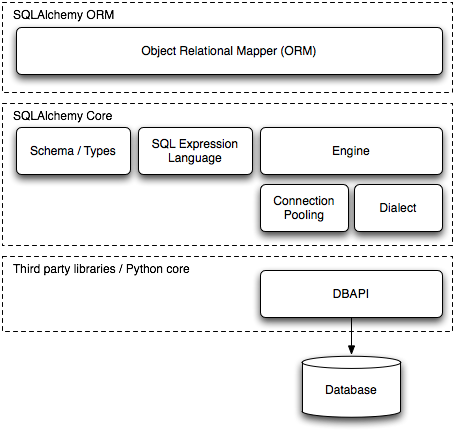
\includegraphics[scale=0.5]{sqla-arch.png}
\end{frame}

\begin{frame}[fragile]{The basics to starts}
\begin{minted}{python}
	""" SQLAlchemy engine factory """
	from sqlalchemy import create_engine
	""" ORM Datatypes """ 
	from sqlalchemy import Column, ForeignKey, Integer, String
	""" ORM Session factory """ 
	from sqlalchemy.orm import sessionmaker
	""" ORM relationship mapper """ 
	from sqlalchemy.orm relationship
	""" Declarative Base Object """ 
	from sqlalchemy.ext.declarative import declarative_base
	""" SQL expresions functions wrappers """ 
	from sqlalchemy.sql import func
\end{minted}
\end{frame}

\begin{frame}[fragile]{Basic Use case}
\begin{minted}{python}
engine = create_engine('sqlite:///demo.db', echo=False)
session = sessionmaker(bind=engine)()
Base.metadata.create_all(engine, checkfirst=True)
p = Parent('prueba')
session.add(p)
session.commit()
\end{minted}
\end{frame}

\begin{frame}[fragile]{Basic Use case}
\begin{minted}{python}
q = session.query(Parent).all()
for x in q:
    c = Child("child", x.id)
    session.add(c)
session.commit()
session.refresh(p)
for x in q:
    print("{}+\n      |".format(x.name))
    for i in x.children:
        print("      +-->{}".format(i.name))
\end{minted}
\end{frame}
\begin{frame}[fragile]{Object mapper and relational pattern}
\textbf{One to Many}
\begin{minted}{python}
Base = declarative_base()

class Parent(Base):
    __tablename__ = 'parent'
    id = Column(Integer, primary_key=True)
    children = relationship("Child", backref="parent")

class Child(Base):
    __tablename__ = 'child'
    id = Column(Integer, primary_key=True)
    parent_id = Column(Integer, ForeignKey('parent.id'))
        
\end{minted}
\end{frame}

\begin{frame}[fragile]{Object mapper and relational pattern}
\textbf{Many to One}
\begin{minted}{python}
class Parent(Base):
    __tablename__ = 'parent'
    id = Column(Integer, primary_key=True)
    child_id = Column(Integer, ForeignKey('child.id'))
    child = relationship("Child")

class Child(Base):
    __tablename__ = 'child'
    id = Column(Integer, primary_key=True)
\end{minted}
\end{frame}

\begin{frame}[fragile]{Object mapper and relational pattern}
\textbf{One to One}
\begin{minted}{python}
class Parent(Base):
    __tablename__ = 'parent'
    id = Column(Integer, primary_key=True)
    child = relationship("Child", uselist=False, 
    						backref="parent")

class Child(Base):
    __tablename__ = 'child'
    id = Column(Integer, primary_key=True)
    parent_id = Column(Integer, ForeignKey('parent.id'))
\end{minted}
\end{frame}

\begin{frame}[fragile]{Object mapper and relational pattern}
\textbf{Many to Many}
\begin{minted}{python}
association_table = Table('association', Base.metadata,
    Column('left_id', Integer, ForeignKey('left.id')),
    Column('right_id', Integer, ForeignKey('right.id'))
)

class Parent(Base):
    __tablename__ = 'left'
    id = Column(Integer, primary_key=True)
    children = relationship("Child",
                    secondary=association_table,
                    backref="parents")

class Child(Base):
    __tablename__ = 'right'
    id = Column(Integer, primary_key=True)
\end{minted}
\end{frame}

\begin{frame}{Bibliography}
\begin{enumerate}
\item SQLAlchemy - Official documentation, March 28, 2014 http://docs.sqlalchemy.org
\item Armin Ronacher - SQLAlchemy and You, July 19, 2011 http://lucumr.pocoo.org/2011/7/19/sqlachemy-and-you/
\item Alexander Solovyov, April 23, 2011 http://solovyov.net/en/2011/basic-sqlalchemy/
\item Alexander Solovyov, May 14, 2012 https://github.com/piranha/slides/blob/gh-pages/sqla-talk/sqla.md
\end{enumerate}
\end{frame}

\begin{frame}{Thanks \& Contact info}
\centering\textbf{Questions?}
\\
\begin{small}
More information or social links about me:\\
http://bsdchile.cl
\end{small}
\end{frame}

%end presentation
\end{document}